\chapterimage{chapter_head_1.jpg} % Chapter heading image

\chapter{What the MCR does for you}

\section{Freshers' Fortnight}
One of the most important things that the MCR does is to provide two weeks of
entertainment and orientation for you when you arrive. Details will be published
when you arrive (both in your pidge and posted around accommodation). The first
event will be held in the Spoom\ref{ssec:Spoom} on Sunday of 0th week (4th
October).
This will be followed by a wide range of events: parties, dinners, pub crawls, quizzes, teas and many more events to help you settle in. It all finishes with the matriculation ceremony on Saturday of 1st week when you formally become part of the University. You do not need to matriculate if you have already studied at Oxford, Cambridge, or Trinity College, Dublin. Remember to wear your sub-fusc and gown to matriculation!

\section{Guest night}
Our main regular social events are \emph{guest nights}. MCR guest nights happen
on Friday of odd weeks so there are four a term. Dinner is usually of a very
high standard and costs \pounds15.55. Members may invite up to four guests to
join them, although many prefer to enjoy the evening with friends from college. Dress is smart, but gowns are not required. After dinner, there are second desserts provided by the MCR which include a selection of cheeses, fruit, chocolate and port, as well as the bar being open. Everyone is welcome to come to this even if you didn't attend the dinner.

Guest nights are very popular and you need to sign-up early on
\url{food.new.ox.ac.uk} to avoid disappointment. Sign-ups start a week early: at
12:01\,am on the preceding Friday.

\section{End-of-term dinners}
The last guest night of term is an end-of-term dinner for which the MCR puts up
a subsidy to make this last dinner extra special. Guests are limited to allow as
many MCR members as possible to attend. Expect a theme, decorations, free drinks and an after-party with a DJ in the MCR.
\enlargethispage{\baselineskip} %Widow avoidance

\section{End-of-year garden party} 
At the end of Trinity term the MCR holds and end-of-year party to say goodbye to the many people leaving Oxford. Enjoy a bouncy castle, games, Pimm's and other summer delights taking you from the day to dancing at night, and pray for good weather! 

\section{Exchange dinners}
We have \emph{exchanges} with other colleges, whereby we host them at New
College for drinks and dinner and then they do the same for us. Drinks and second desserts are included. These events vary between being a special dinner with high table food or occurring during regular formal dinners. The MCR also tries to do an exchange with a Cambridge college once a year. 

\section{Brunch}
During term, and occasionally out of term, the MCR hosts a free brunch in the
Spoom on Sunday mornings at 11\,am. This is a good way to catch up with friends and meet new people. Arrive early to avoid missing out on the smoked salmon!

\begin{figure}[htbp]
\centering
		\begin{minipage}{0.45\textwidth}
			\centering
				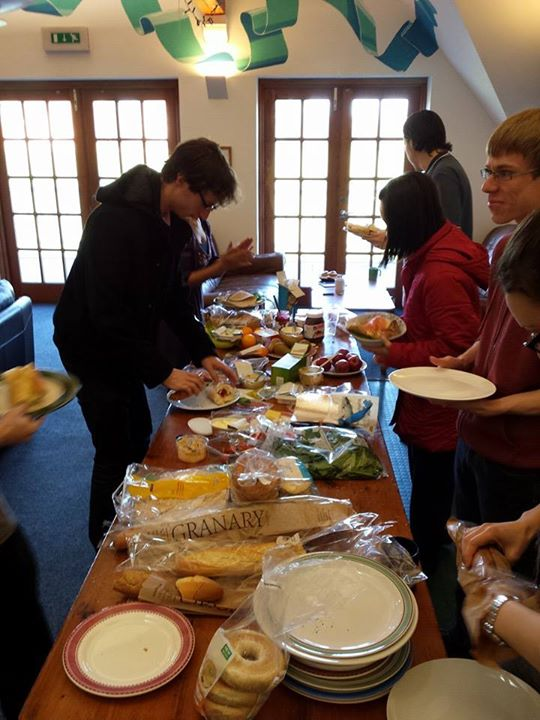
\includegraphics[width=0.9\textwidth]{brunch.jpg}
				\caption[]{A brunch in the Spoom}
                \label{fig:brunch}
        \end{minipage}%
        \quad
        \begin{minipage}{0.45\textwidth}
        	\centering
				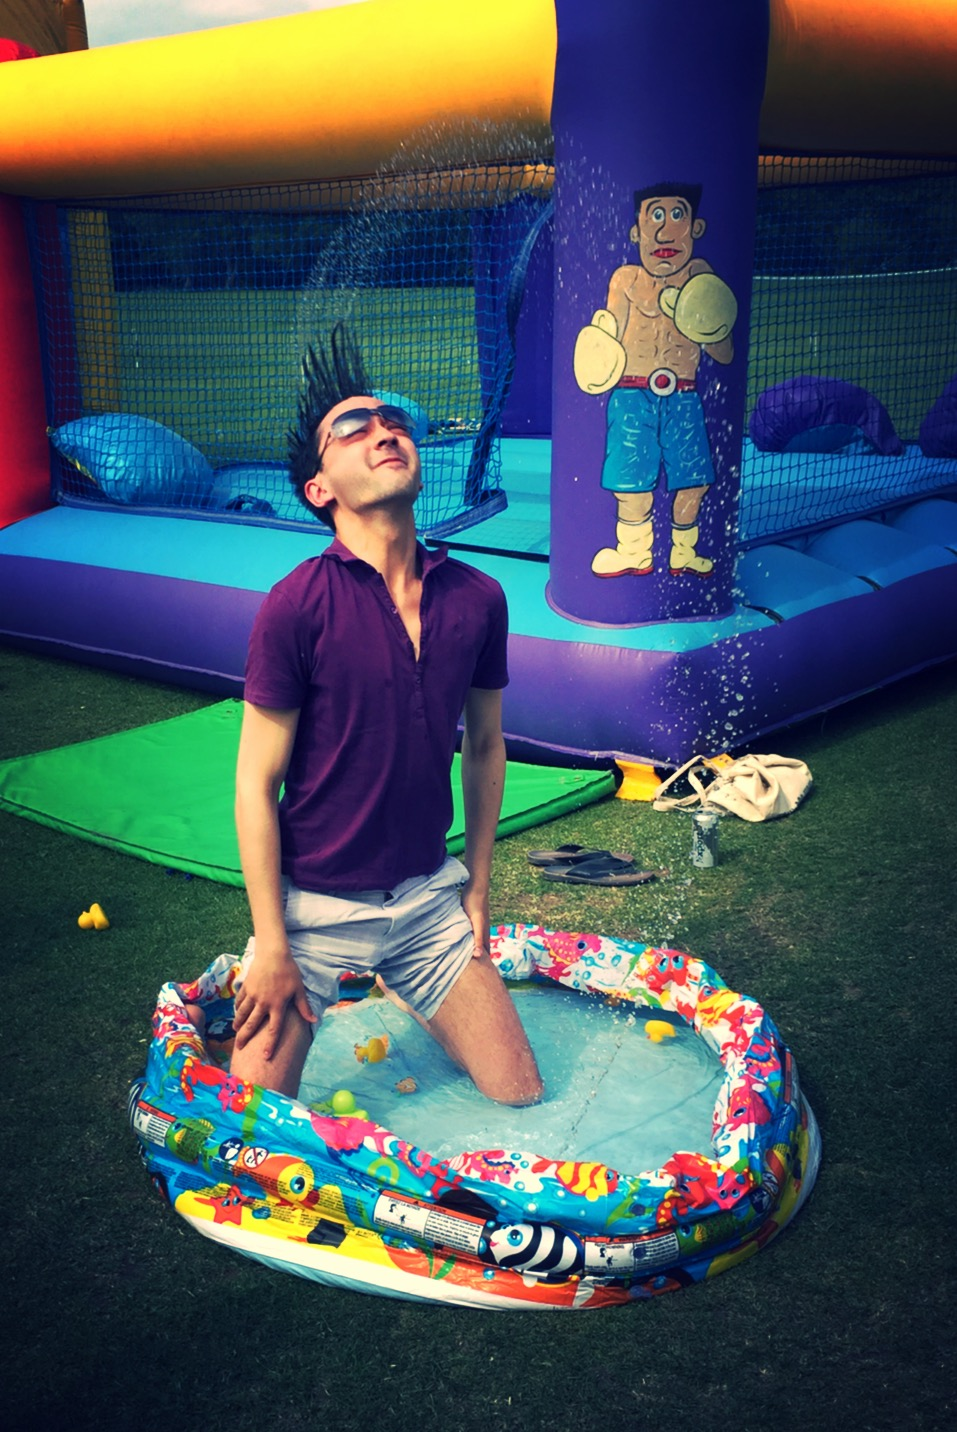
\includegraphics[width=0.9\textwidth]{eoyp.jpg}
				\caption[]{Typical scene at the
				garden party}
				\label{fig:eoyp}
        \end{minipage}%
\end{figure}

\section{Bar Nights}
During term the MCR opens the bar between 9.00-11.00\,pm on a Wednesday and
Thursday. The bar is also open on alternate Friday evenings and the occasional Saturday evening.


\begin{figure}[htbp]
\centering
		\begin{minipage}{0.45\textwidth}
				\centering
				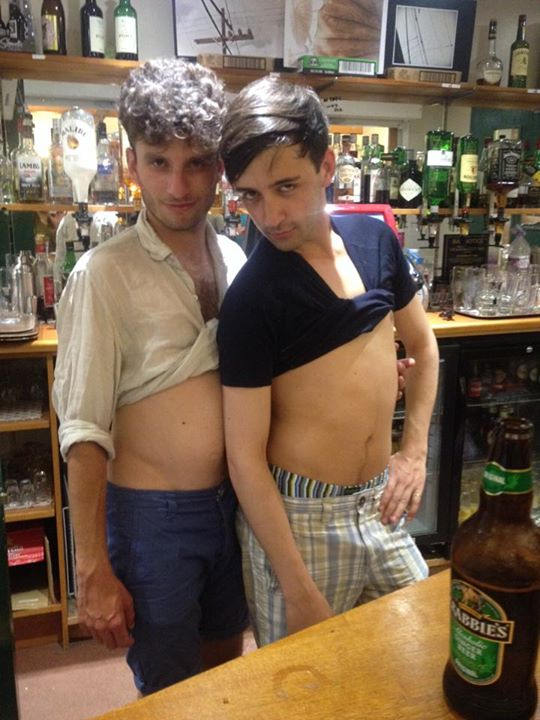
\includegraphics[width=.8\textwidth]{bar.jpg}
				\caption[]{Absolutely typical bar night}
				\label{fig:bar}
        \end{minipage}%
        \quad
        \begin{minipage}{0.45\textwidth}
				\centering
				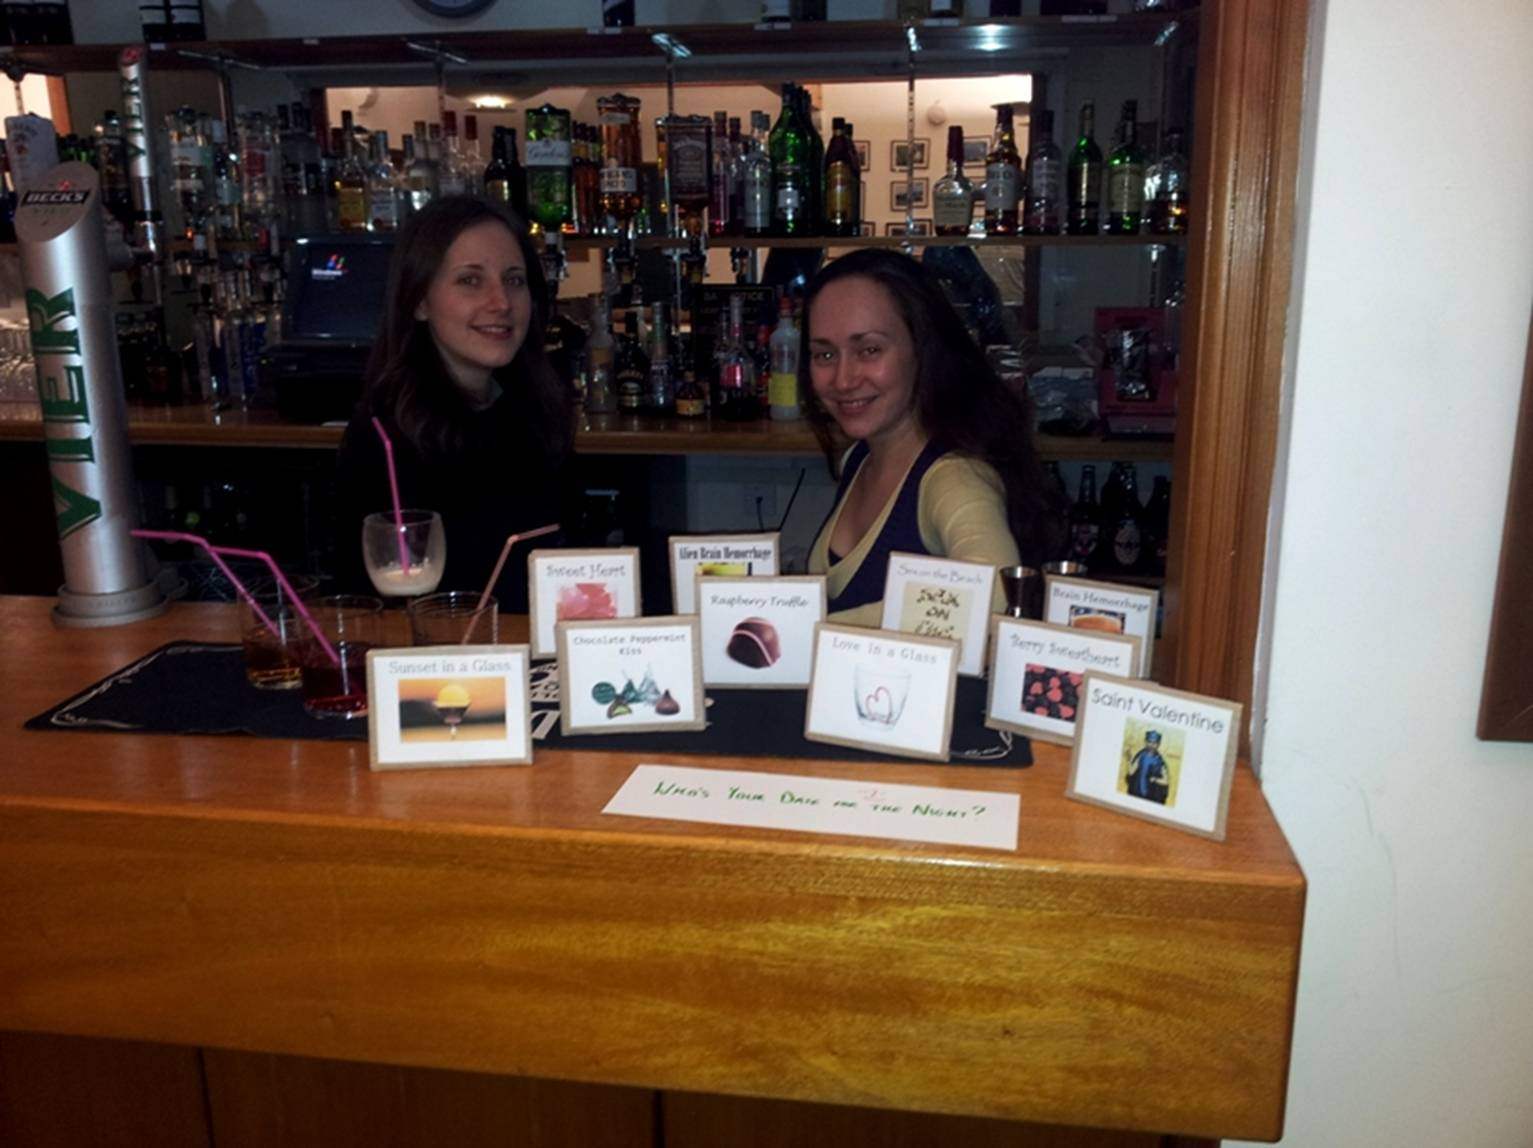
\includegraphics[width=.8\textwidth]{bar2.jpg}
				\caption[]{A bop}
				\label{fig:bop}
        \end{minipage}%
\end{figure}

\section{Bops}
Bops are the highlight of the MCR party scene. Around once a term the MCR will
throw parties with a fun theme and a DJ in the Spoom. They normally occur after guest night dinners and the bar remains open later than usual. Other colleges also host their own Bops located on their grounds, which you are welcome to attend if advertised. 

\section{New Collection}
The MCR's own multi-disciplinary academic journal, The New Collection, aims to present the breadth and depth of work currently being undertaken by the graduate members of New College. All work contained within the journal is by current graduate MCR members and every MCR member is encouraged to get involved by either submitting an article or during the editorial phase.

The New Collection provides members the unique opportunity of learning both how to write and review journal articles all within the supportive structure of New College, making us the envy of other colleges. Successful articles this year came from a variety of disciplines and were aimed at a broad readership, which is the original aim of the New Collection - to bring the current work of our MCR members to a larger intellectual audience.

\section{Colloquia}
Each term, members of the MCR are invited to present their research in colloquia. Around 2009, we introduced a new tradition, collaborating with the SCR for the first time. The colloquia comprise a 20-30 minute talk by a graduate student, followed by a response from a member of the SCR working in the same field. The floor is then opened to general questions and discussion, with members from not just the MCR, but also JCR and SCR invited to attend. These talks are an excellent opportunity to gain presentation experience, but more importantly the Graduate Colloquia are the cornerstone of our intellectual engagement with College. The atmosphere is informal and supportive, and offers a chance to learn what it is your peers may be working on in labs and libraries when away from Weston and the Spoom! The new SCR involvement also offers a great chance to get expert feedback on your work from someone other than your supervisor. Past colloquia have covered topics ranging from The Universe, to Crime fiction. The goal is to present an academic topic in which you are presently immersed to an audience who may or may not have experience of the concepts.

The MCR Vice-President organizes the colloquia and is always seeking MCR members
willing to present a colloquium, so please consider doing so, emailing Tanja
Collavo
(\href{mailto:tanja.collavo@new.ox.ac.uk}{\urlformat{tanja.collavo@new.ox.ac.uk}})
if you are interested.

Since last year, a fervour forum has been introduced as well, always organized
by the MCR Vice-President The Fervour Forum consists of 5\,minutes
presentations/demonstrations of an MCR member's hobby or passion and followed by 5-10 minutes Q\&A. Usually there are 3-4 presentations in the same way and they represent a great way to know better other MCR members and learn new, funny and interesting things.

\section{The MCR play}
The Arts and Culture organizes every year a theatre played performed in Trinity
term either in the college garden or cloisters. Actors and Production team are
selected primarily from volunteers from the MCR. The play is usually on stage for an entire weekend and requires around six weeks of preparation and rehearsals. In 2015 the MCR produced Hay Fever, a comedy set in the '20s, obtaining a great success across both college and non-college audiences. If you want to be involved with the next MCR theatre play, get in touch with Dionysios (\href{mailto:dionysios.kyropoulos@music.ox.ac.uk}{\urlformat{dionysios.kyropoulos@music.ox.ac.uk}}).

\begin{figure}[htbp]
\centering
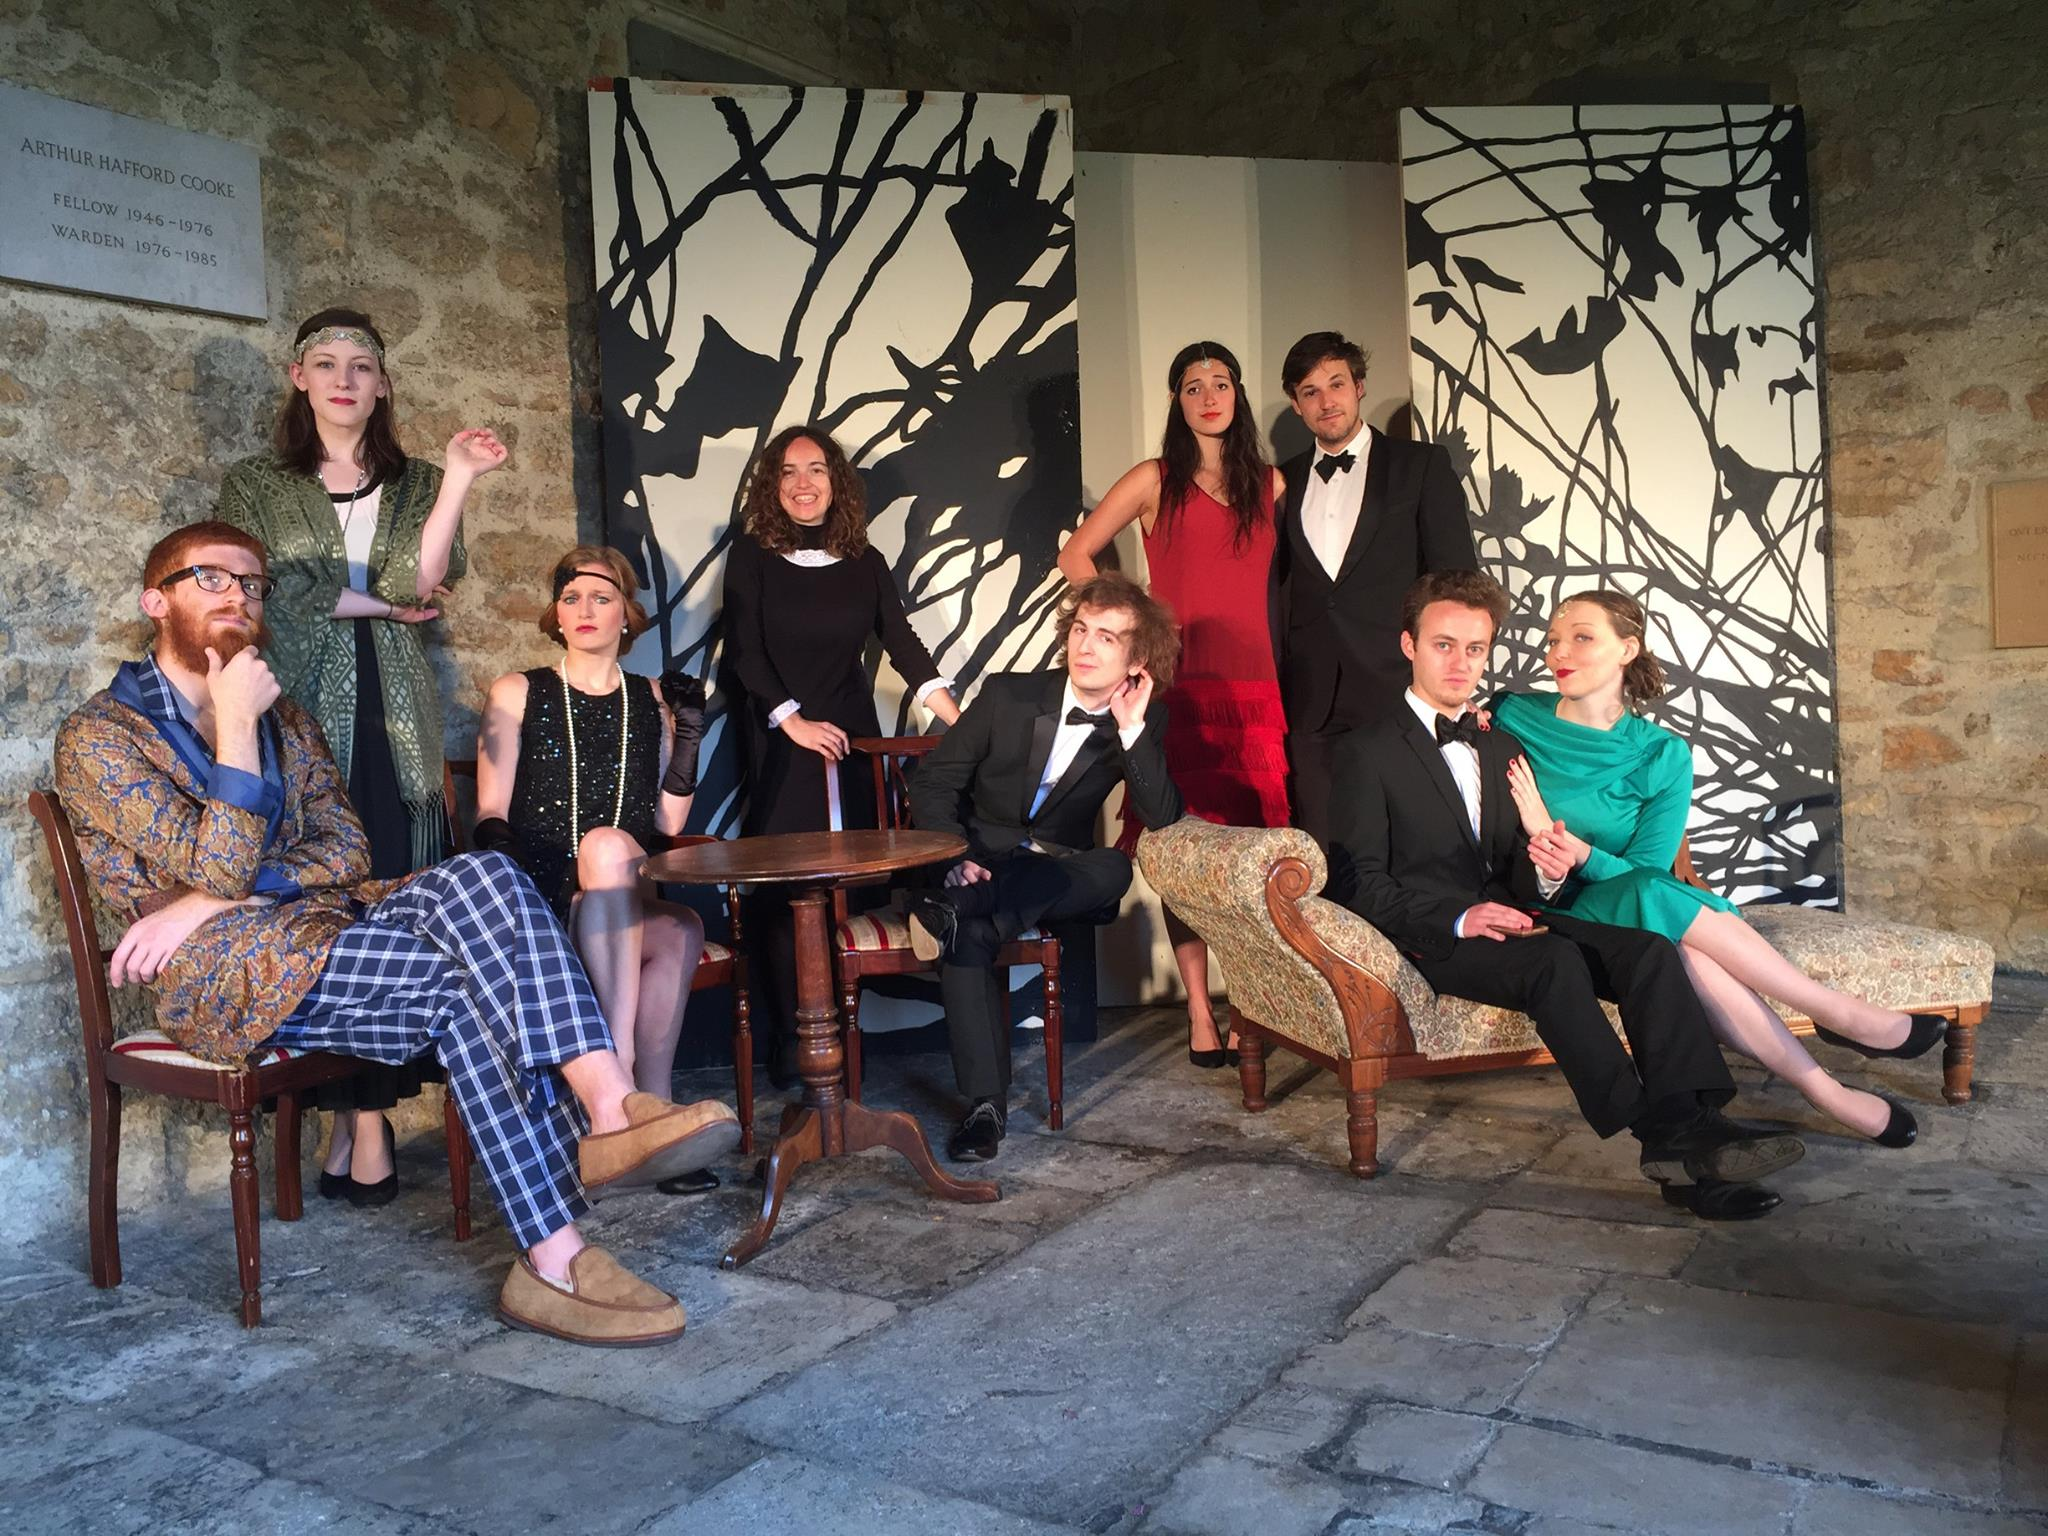
\includegraphics[width=0.75\textwidth]{play.jpg}
\caption[]{The 2015 MCR play,
\emph{Hay Fever}}
\label{fig:play}
\end{figure}

\section{Other events}
The MCR puts on several other events during the term in addition to the regulars. These include orchestral concert trips, MCR quizzes, a play, cheese and wine tasting, etc. These occur regularly throughout term, so keep an eye on the MCR mailing list and Facebook page for adverts.


\begin{figure}[htbp]
\centering
		\begin{minipage}{0.3\textwidth}
                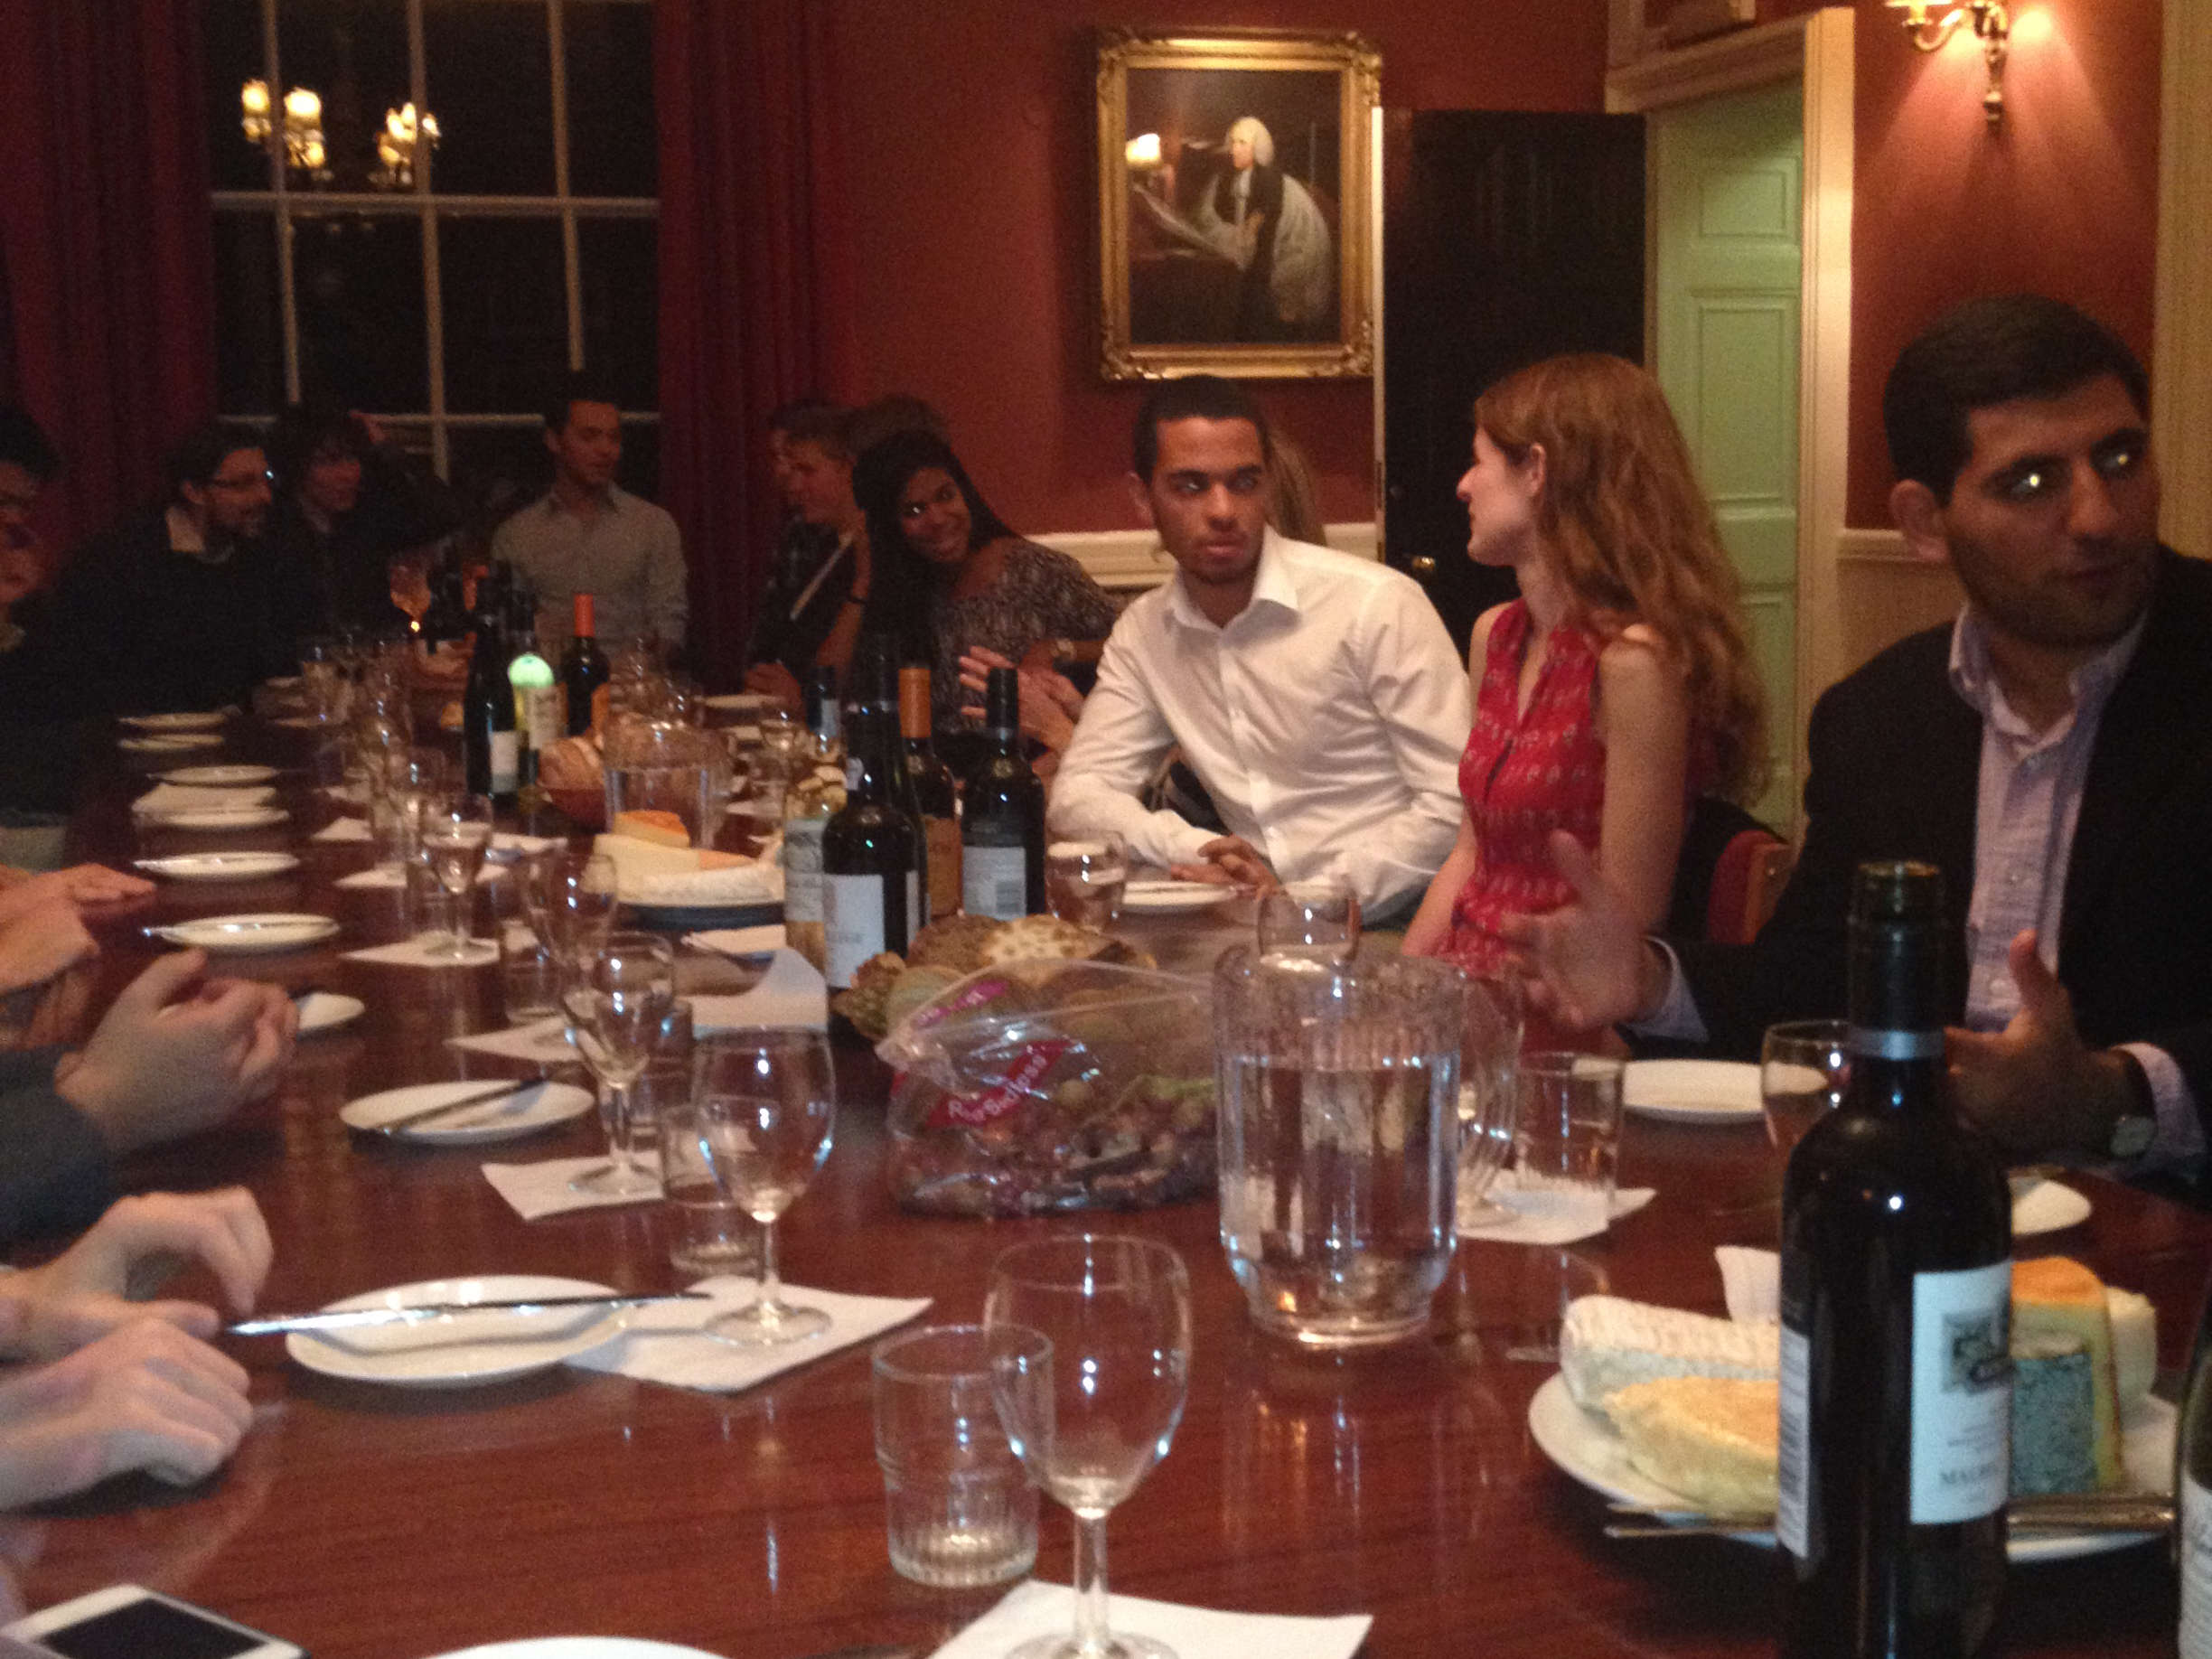
\includegraphics[width=\textwidth]{cheese2.jpg}
                \caption[]{Cheese and Wine tasting}
                \label{fig:cheese}
        \end{minipage}%
        \quad
        \begin{minipage}{0.3\textwidth}
                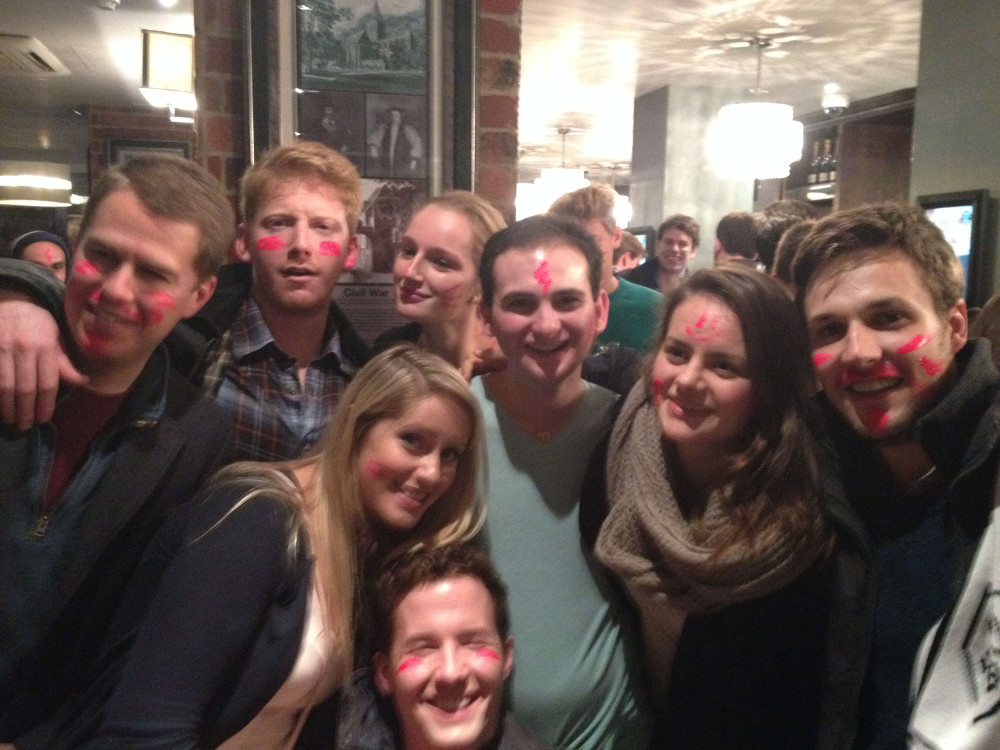
\includegraphics[width= \textwidth]{pub.jpg}
                \caption[]{Freshers' Week Pub Crawl}
                \label{fig:crawl}
        \end{minipage}%
        \quad
        \begin{minipage}{0.30\textwidth}      
                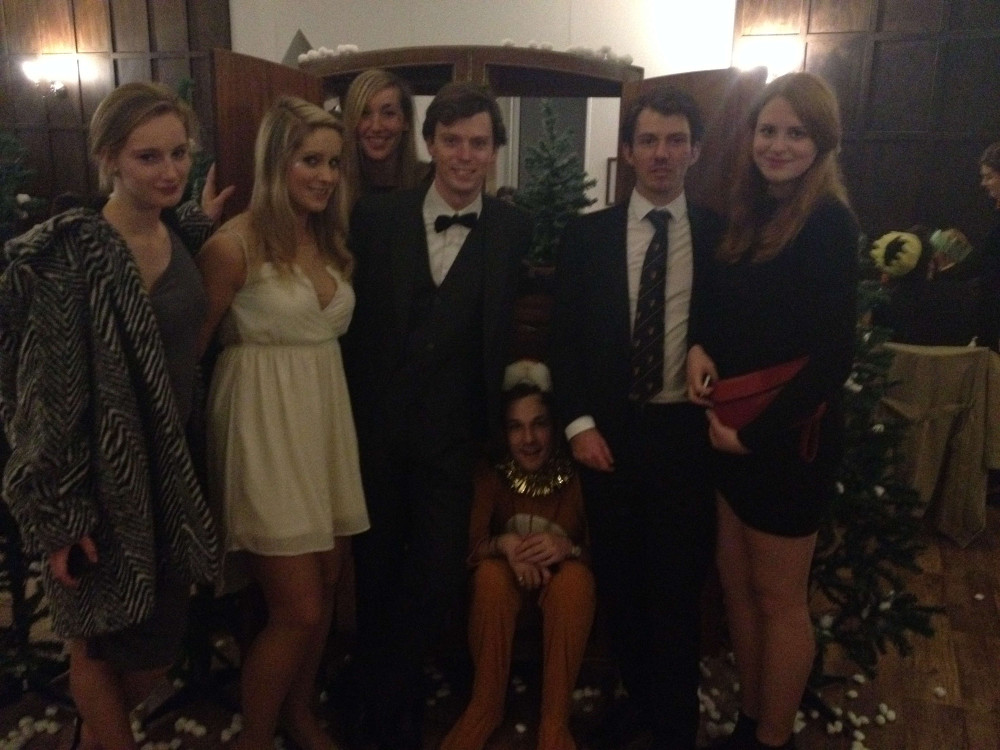
\includegraphics[width= \textwidth]{narnia.jpg}
                \caption[]{Narnia-themed End-of-term Dinner}
                \label{fig:narnia}
        \end{minipage}%
\end{figure}